\documentclass{standalone}
\usepackage{tikz}
\usetikzlibrary{patterns, positioning}


\begin{document}
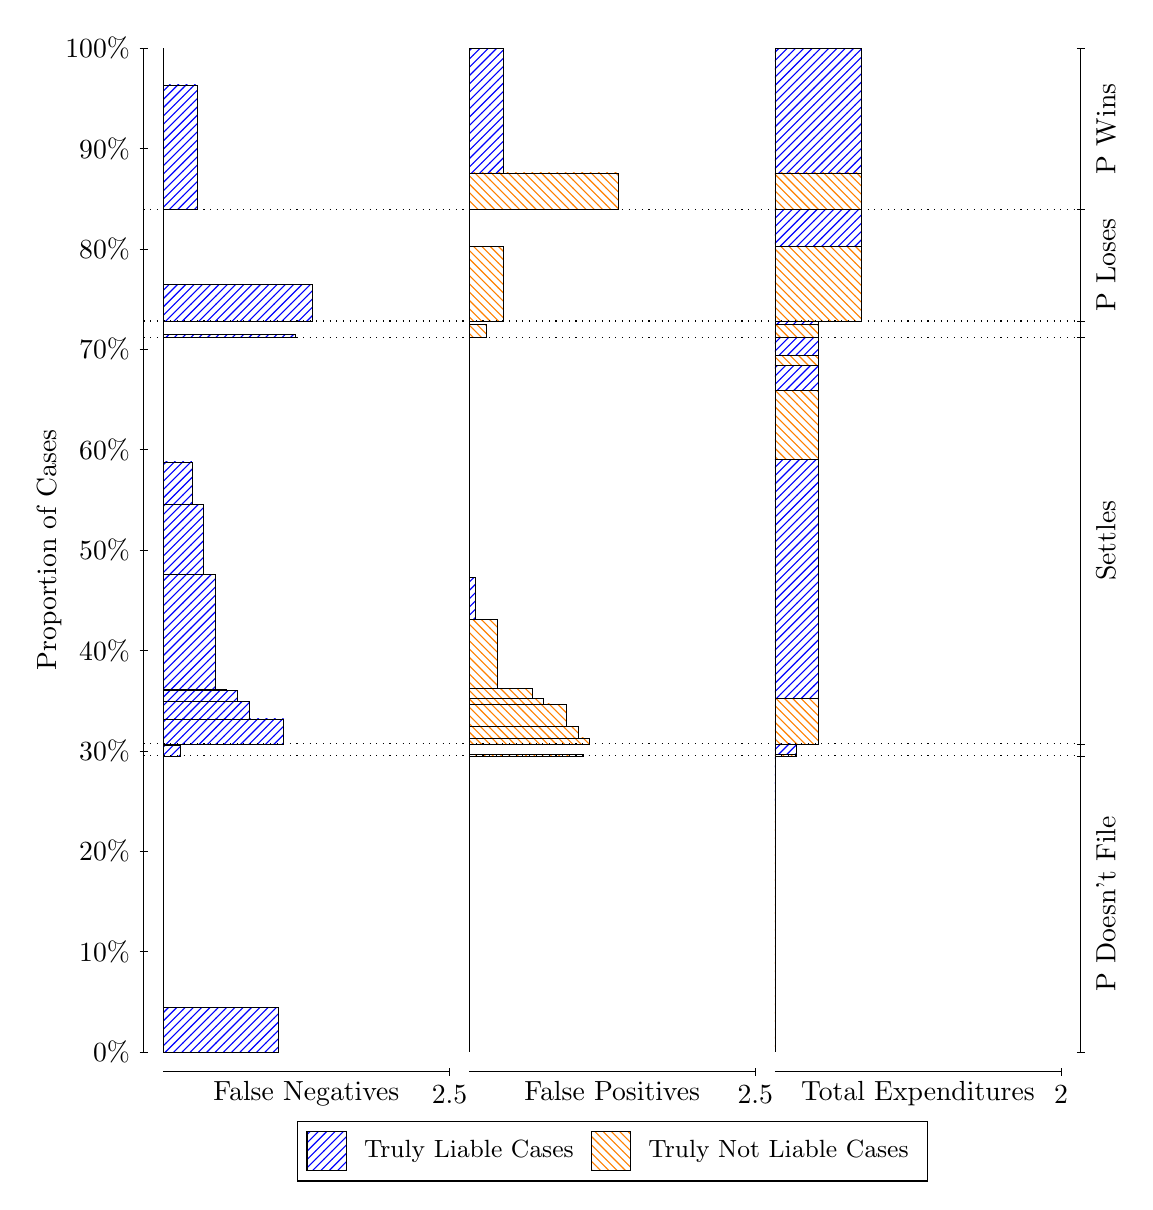
\begin{tikzpicture}
\draw[black, very thin] (1.5,1.75) -- (1.5,14.5);
\node[rotate=90, text=black, anchor=center] at (0.3, 8.125) {Proportion of Cases};
\draw[black, very thin] (1.45,1.75) -- (1.55,1.75);
\node[text=black, anchor=east] at (1.45, 1.75) {0\%};
\draw[black, very thin] (1.45,3.025) -- (1.55,3.025);
\node[text=black, anchor=east] at (1.45, 3.025) {10\%};
\draw[black, very thin] (1.45,4.3) -- (1.55,4.3);
\node[text=black, anchor=east] at (1.45, 4.3) {20\%};
\draw[black, very thin] (1.45,5.575) -- (1.55,5.575);
\node[text=black, anchor=east] at (1.45, 5.575) {30\%};
\draw[black, very thin] (1.45,6.85) -- (1.55,6.85);
\node[text=black, anchor=east] at (1.45, 6.85) {40\%};
\draw[black, very thin] (1.45,8.125) -- (1.55,8.125);
\node[text=black, anchor=east] at (1.45, 8.125) {50\%};
\draw[black, very thin] (1.45,9.4) -- (1.55,9.4);
\node[text=black, anchor=east] at (1.45, 9.4) {60\%};
\draw[black, very thin] (1.45,10.675) -- (1.55,10.675);
\node[text=black, anchor=east] at (1.45, 10.675) {70\%};
\draw[black, very thin] (1.45,11.95) -- (1.55,11.95);
\node[text=black, anchor=east] at (1.45, 11.95) {80\%};
\draw[black, very thin] (1.45,13.225) -- (1.55,13.225);
\node[text=black, anchor=east] at (1.45, 13.225) {90\%};
\draw[black, very thin] (1.45,14.5) -- (1.55,14.5);
\node[text=black, anchor=east] at (1.45, 14.5) {100\%};

\draw[black, very thin] (13.4,1.75) -- (13.4,14.5);
\draw[black, very thin] (13.35,1.75) -- (13.45,1.75);
\node[anchor=west] at (13.35, 1.75) {};
\draw[black, very thin] (13.35,5.5102) -- (13.45,5.5102);
\node[anchor=west] at (13.35, 5.5102) {};
\draw[black, very thin] (13.35,5.6636) -- (13.45,5.6636);
\node[anchor=west] at (13.35, 5.6636) {};
\draw[black, very thin] (13.35,10.825) -- (13.45,10.825);
\node[anchor=west] at (13.35, 10.825) {};
\draw[black, very thin] (13.35,11.033) -- (13.45,11.033);
\node[anchor=west] at (13.35, 11.033) {};
\draw[black, very thin] (13.35,12.449) -- (13.45,12.449);
\node[anchor=west] at (13.35, 12.449) {};
\draw[black, very thin] (13.35,14.5) -- (13.45,14.5);
\node[anchor=west] at (13.35, 14.5) {};

\draw[black, very thin, pattern color=blue, pattern=north east lines] (1.75,1.75) rectangle (3.2033,2.3198);
\draw[black, very thin, pattern color=orange, pattern=north west lines] (1.75,2.3198) rectangle (1.75,5.5102);
\draw[black, very thin, pattern color=blue, pattern=north east lines] (1.75,5.5102) rectangle (1.968,5.6486);
\draw[black, very thin, pattern color=orange, pattern=north west lines] (1.75,5.6486) rectangle (1.75,5.6636);
\draw[black, very thin, pattern color=blue, pattern=north east lines] (1.75,5.6636) rectangle (3.276,5.9794);
\draw[black, very thin, pattern color=blue, pattern=north east lines] (1.75,5.9794) rectangle (2.84,6.2064);
\draw[black, very thin, pattern color=blue, pattern=north east lines] (1.75,6.2064) rectangle (2.6947,6.344);
\draw[black, very thin, pattern color=blue, pattern=north east lines] (1.75,6.344) rectangle (2.5493,6.3561);
\draw[black, very thin, pattern color=blue, pattern=north east lines] (1.75,6.3561) rectangle (2.404,7.8113);
\draw[black, very thin, pattern color=blue, pattern=north east lines] (1.75,7.8113) rectangle (2.2587,8.7092);
\draw[black, very thin, pattern color=blue, pattern=north east lines] (1.75,8.7092) rectangle (2.1133,9.2437);
\draw[black, very thin, pattern color=orange, pattern=north west lines] (1.75,9.2437) rectangle (1.75,10.825);
\draw[black, very thin, pattern color=blue, pattern=north east lines] (1.75,10.825) rectangle (3.4213,10.863);
\draw[black, very thin, pattern color=orange, pattern=north west lines] (1.75,10.863) rectangle (1.75,11.033);
\draw[black, very thin, pattern color=blue, pattern=north east lines] (1.75,11.033) rectangle (3.6393,11.497);
\draw[black, very thin, pattern color=orange, pattern=north west lines] (1.75,11.497) rectangle (1.75,12.449);
\draw[black, very thin, pattern color=blue, pattern=north east lines] (1.75,12.449) rectangle (2.186,14.033);
\draw[black, very thin, pattern color=orange, pattern=north west lines] (1.75,14.033) rectangle (1.75,14.5);
\draw[black, very thin, pattern color=orange, pattern=north west lines] (5.6333,1.75) rectangle (5.6333,4.9404);
\draw[black, very thin, pattern color=blue, pattern=north east lines] (5.6333,4.9404) rectangle (5.6333,5.5102);
\draw[black, very thin, pattern color=orange, pattern=north west lines] (5.6333,5.5102) rectangle (7.0867,5.5253);
\draw[black, very thin, pattern color=blue, pattern=north east lines] (5.6333,5.5253) rectangle (5.6333,5.6636);
\draw[black, very thin, pattern color=orange, pattern=north west lines] (5.6333,5.6636) rectangle (7.1593,5.7375);
\draw[black, very thin, pattern color=orange, pattern=north west lines] (5.6333,5.7375) rectangle (7.014,5.8811);
\draw[black, very thin, pattern color=orange, pattern=north west lines] (5.6333,5.8811) rectangle (6.8687,6.1595);
\draw[black, very thin, pattern color=orange, pattern=north west lines] (5.6333,6.1595) rectangle (6.7233,6.172);
\draw[black, very thin, pattern color=orange, pattern=north west lines] (5.6333,6.172) rectangle (6.578,6.2367);
\draw[black, very thin, pattern color=orange, pattern=north west lines] (5.6333,6.2367) rectangle (6.4327,6.3629);
\draw[black, very thin, pattern color=orange, pattern=north west lines] (5.6333,6.3629) rectangle (5.9967,7.2444);
\draw[black, very thin, pattern color=blue, pattern=north east lines] (5.6333,7.2444) rectangle (5.706,7.779);
\draw[black, very thin, pattern color=blue, pattern=north east lines] (5.6333,7.779) rectangle (5.6333,10.825);
\draw[black, very thin, pattern color=orange, pattern=north west lines] (5.6333,10.825) rectangle (5.8513,10.995);
\draw[black, very thin, pattern color=blue, pattern=north east lines] (5.6333,10.995) rectangle (5.6333,11.033);
\draw[black, very thin, pattern color=orange, pattern=north west lines] (5.6333,11.033) rectangle (6.0693,11.985);
\draw[black, very thin, pattern color=blue, pattern=north east lines] (5.6333,11.985) rectangle (5.6333,12.449);
\draw[black, very thin, pattern color=orange, pattern=north west lines] (5.6333,12.449) rectangle (7.5227,12.915);
\draw[black, very thin, pattern color=blue, pattern=north east lines] (5.6333,12.915) rectangle (6.0693,14.5);
\draw[black, very thin, pattern color=orange, pattern=north west lines] (9.5167,1.75) rectangle (9.5167,4.9404);
\draw[black, very thin, pattern color=blue, pattern=north east lines] (9.5167,4.9404) rectangle (9.5167,5.5102);
\draw[black, very thin, pattern color=orange, pattern=north west lines] (9.5167,5.5102) rectangle (9.7892,5.5253);
\draw[black, very thin, pattern color=blue, pattern=north east lines] (9.5167,5.5253) rectangle (9.7892,5.6636);
\draw[black, very thin, pattern color=orange, pattern=north west lines] (9.5167,5.6636) rectangle (10.062,6.2367);
\draw[black, very thin, pattern color=blue, pattern=north east lines] (9.5167,6.2367) rectangle (10.062,9.274);
\draw[black, very thin, pattern color=orange, pattern=north west lines] (9.5167,9.274) rectangle (10.062,10.156);
\draw[black, very thin, pattern color=blue, pattern=north east lines] (9.5167,10.156) rectangle (10.062,10.471);
\draw[black, very thin, pattern color=orange, pattern=north west lines] (9.5167,10.471) rectangle (10.062,10.598);
\draw[black, very thin, pattern color=blue, pattern=north east lines] (9.5167,10.598) rectangle (10.062,10.825);
\draw[black, very thin, pattern color=orange, pattern=north west lines] (9.5167,10.825) rectangle (10.062,10.995);
\draw[black, very thin, pattern color=blue, pattern=north east lines] (9.5167,10.995) rectangle (10.062,11.033);
\draw[black, very thin, pattern color=orange, pattern=north west lines] (9.5167,11.033) rectangle (10.607,11.985);
\draw[black, very thin, pattern color=blue, pattern=north east lines] (9.5167,11.985) rectangle (10.607,12.449);
\draw[black, very thin, pattern color=orange, pattern=north west lines] (9.5167,12.449) rectangle (10.607,12.915);
\draw[black, very thin, pattern color=blue, pattern=north east lines] (9.5167,12.915) rectangle (10.607,14.5);
\draw[black, dotted] (1.5,5.5102) -- (13.4,5.5102);
\draw[black, dotted] (1.5,5.6636) -- (13.4,5.6636);
\draw[black, dotted] (1.5,10.825) -- (13.4,10.825);
\draw[black, dotted] (1.5,11.033) -- (13.4,11.033);
\draw[black, dotted] (1.5,12.449) -- (13.4,12.449);
\draw[black, very thin] (1.75,1.5) -- (5.3833,1.5);
\node[text=black, anchor=north] at (3.5667, 1.5) {False Negatives};
\draw[black, very thin] (5.3833,1.45) -- (5.3833,1.55);
\node[text=black, anchor=north] at (5.3833, 1.45) {2.5};

\draw[black, very thin] (5.6333,1.5) -- (9.2667,1.5);
\node[text=black, anchor=north] at (7.45, 1.5) {False Positives};
\draw[black, very thin] (9.2667,1.45) -- (9.2667,1.55);
\node[text=black, anchor=north] at (9.2667, 1.45) {2.5};

\draw[black, very thin] (9.5167,1.5) -- (13.15,1.5);
\node[text=black, anchor=north] at (11.333, 1.5) {Total Expenditures};
\draw[black, very thin] (13.15,1.45) -- (13.15,1.55);
\node[text=black, anchor=north] at (13.15, 1.45) {2};

\node[text=black, centered, rotate=90] at (13.72, 3.6301) {P Doesn't File};

\node[text=black, centered, rotate=90] at (13.72, 8.2441) {Settles};

\node[text=black, centered, rotate=90] at (13.72, 11.741) {P Loses};
\node[text=black, centered, rotate=90] at (13.72, 13.474) {P Wins};

\draw (7.449999999999999,1.5) node[draw=none] (baseCoordinate) {};
\begin{scope}[align=center]
        \matrix[scale=0.5, draw=black, below=0.5cm of baseCoordinate, nodes={draw}, column sep=0.1cm]{
            \node[rectangle, draw, minimum width=0.5cm, minimum height=0.5cm, pattern color=blue, pattern=north east lines] {}; &
            \node[draw=none, font=\small, text=black] (B) {Truly Liable Cases}; &
            \node[rectangle, draw, minimum width=0.5cm, minimum height=0.5cm, pattern color=orange, pattern=north west lines] {}; &
            \node[draw=none, font=\small, text=black] (B) {Truly Not Liable Cases}; \\
            };
\end{scope}

\end{tikzpicture}
\end{document}